%
% abstand.tex
%
% (c) 2018 Prof Dr Andreas Müller, Hochschule Rapperswil
%
\documentclass[tikz]{standalone}
\usepackage{times}
\usepackage{amsmath}
\usepackage{txfonts}
\usepackage[utf8]{inputenc}
\usepackage{graphics}
\usetikzlibrary{arrows,intersections,math}
\usepackage{ifthen}
\begin{document}

\newboolean{showgrid}
\setboolean{showgrid}{false}

\begin{tikzpicture}[>=latex,thick]

% Povray Bild
\node at (0,0) {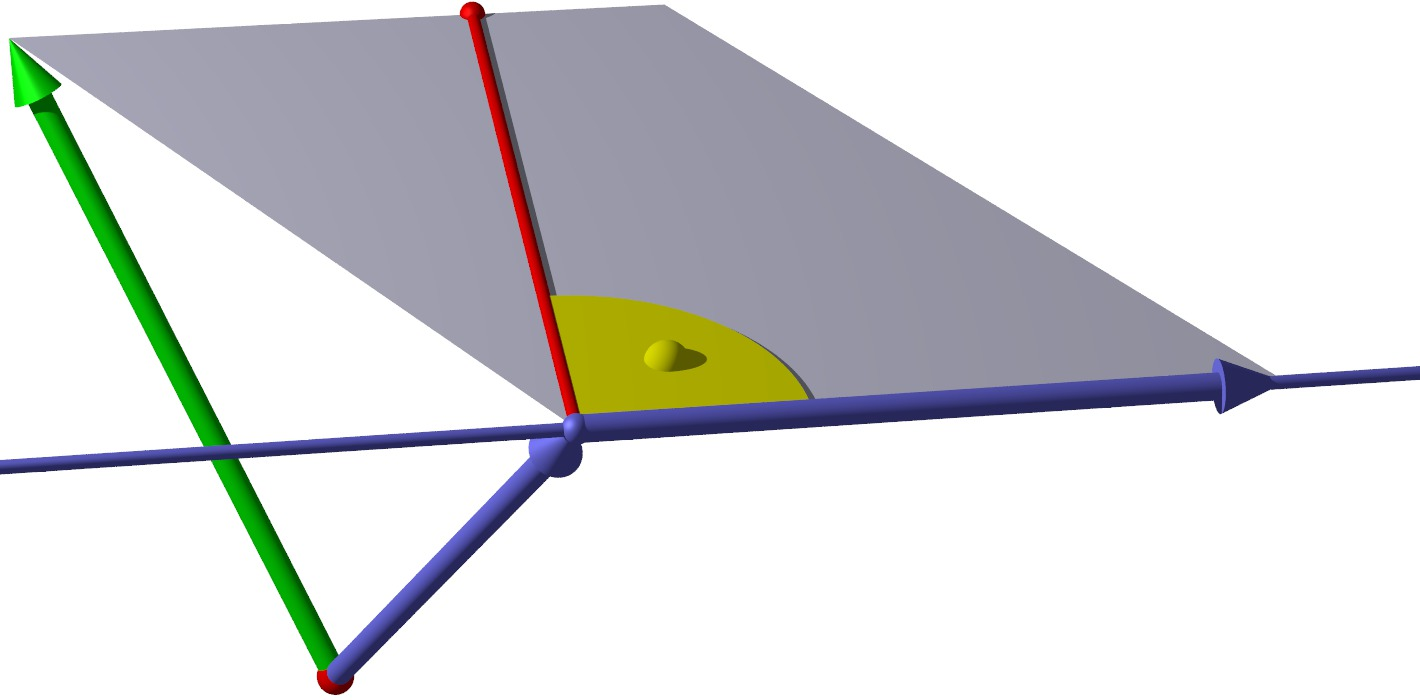
\includegraphics[width=10cm]{abstand.jpg}};

% Gitter
\ifthenelse{\boolean{showgrid}}{
\draw[step=0.1,line width=0.1pt] (-5,-3) grid (5, 3);
\draw[step=0.5,line width=0.4pt] (-5,-3) grid (5, 3);
\draw (-5,-3) grid (5, 3);
\fill (0,0) circle[radius=0.05];
}{}

% Gerade
\node at (4,-0.6) {$\vec{r}$};
\node at (-0.7,-0.9) {$P$};
\node at (-1.5,-1.6) {$\vec{p}$};

% Nullpunkt
\node at (-2.4,-2.5) {$O$};

% Höhe
\node at (-1.1,1.7) {$h$};

% Punkt a
\node at (-4.8,2.5) {$A$};
\node at (-4.7,1) {$\vec{a}$};

% Flächeninhalt
\node at (0.6,0.6) {$F=|\vec{r}\times(\vec{a}-\vec{p})|=h\cdot|\vec{r}|$};

\end{tikzpicture}

\end{document}

